\section{The negative loop archetype}
\begin{frame}
  \frametitle{The negative loop archetype}

  \begin{definition}[Negative loop archetype]
    Two neurons where the first receives the input signal and an inhibition from the second and the second is activated by the first.
  \end{definition}

  \begin{columns}
    \begin{column}{0.45\textwidth}
      \begin{figure}
        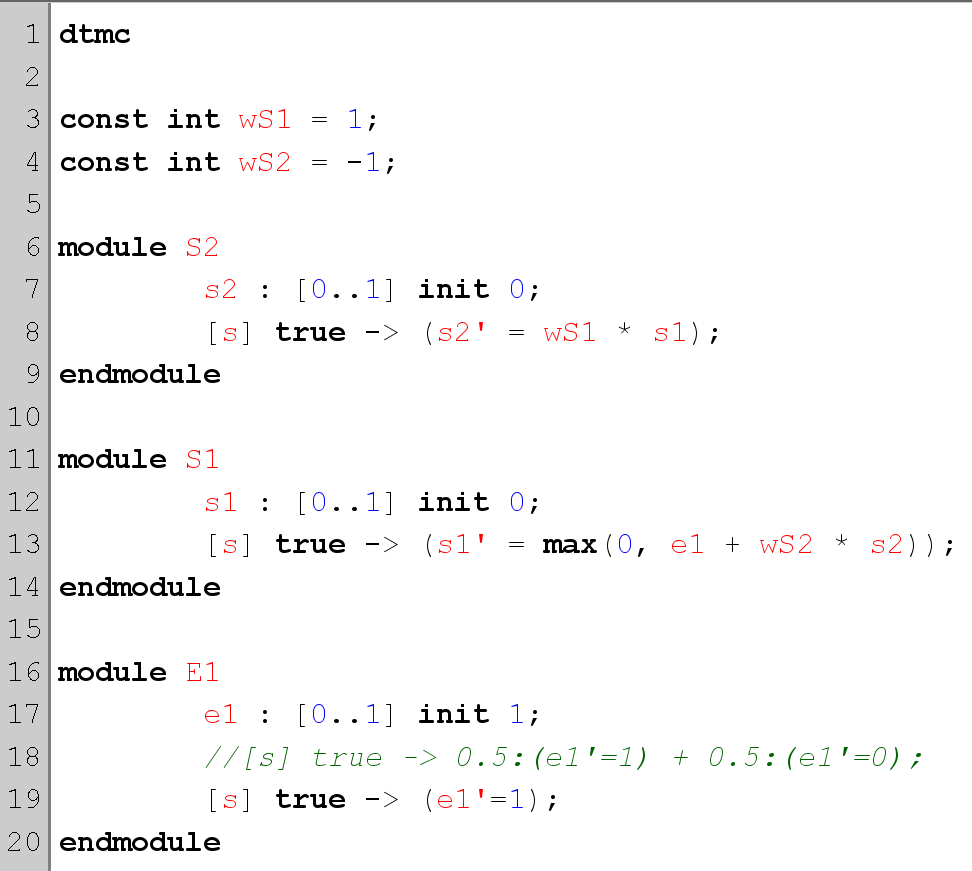
\includegraphics[width=1\textwidth]{pic/neg_loop_simple.png}
      \end{figure}
    \end{column}
    \begin{column}{0.45\textwidth}
      \begin{remark}
        Note the max function $\rightarrow$ the signal of $S1$ can only be $0$ or $1$.
      \end{remark}
    \end{column}
  \end{columns}

\end{frame}

\begin{frame}
  \frametitle{A plot of negative loop}

  \begin{figure}
    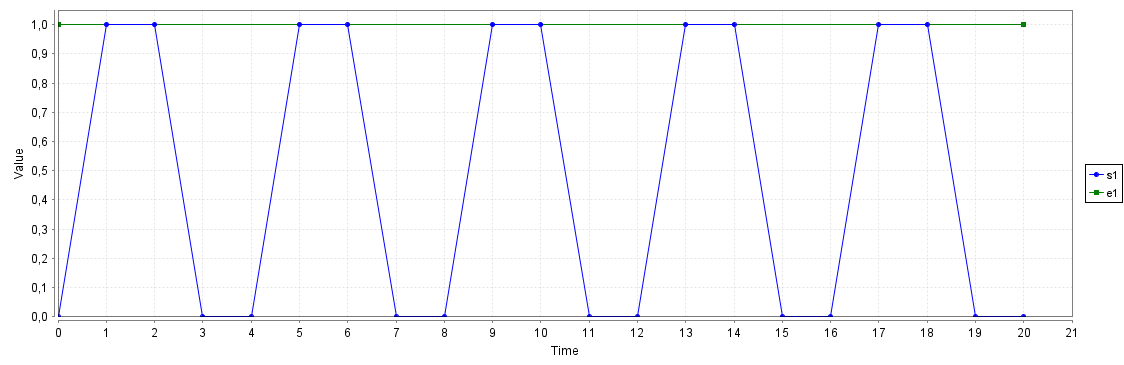
\includegraphics[width=\textwidth]{pic/neg_loop_simple_plot_1.png}
  \end{figure}

  Some properties:
  \begin{itemize}
    \item $P = [ G (e_1=1) ] ?$ \uncover<2->{$1.0$}
    \item $P = [ G ((s_2=1 \land (X s_2=1)) \Rightarrow (X X s_2=0))] ?$ \uncover<3->{$1.0$}
    \item $P = [ G ((s_2=0 \land (X s_2=0)) \Rightarrow (X X s_2=1))] ?$ \uncover<4->{$1.0$}
  \end{itemize}

\end{frame}

% \begin{frame}
%   \frametitle{Negative loop in LI\&F style}

%   \begin{figure}
%     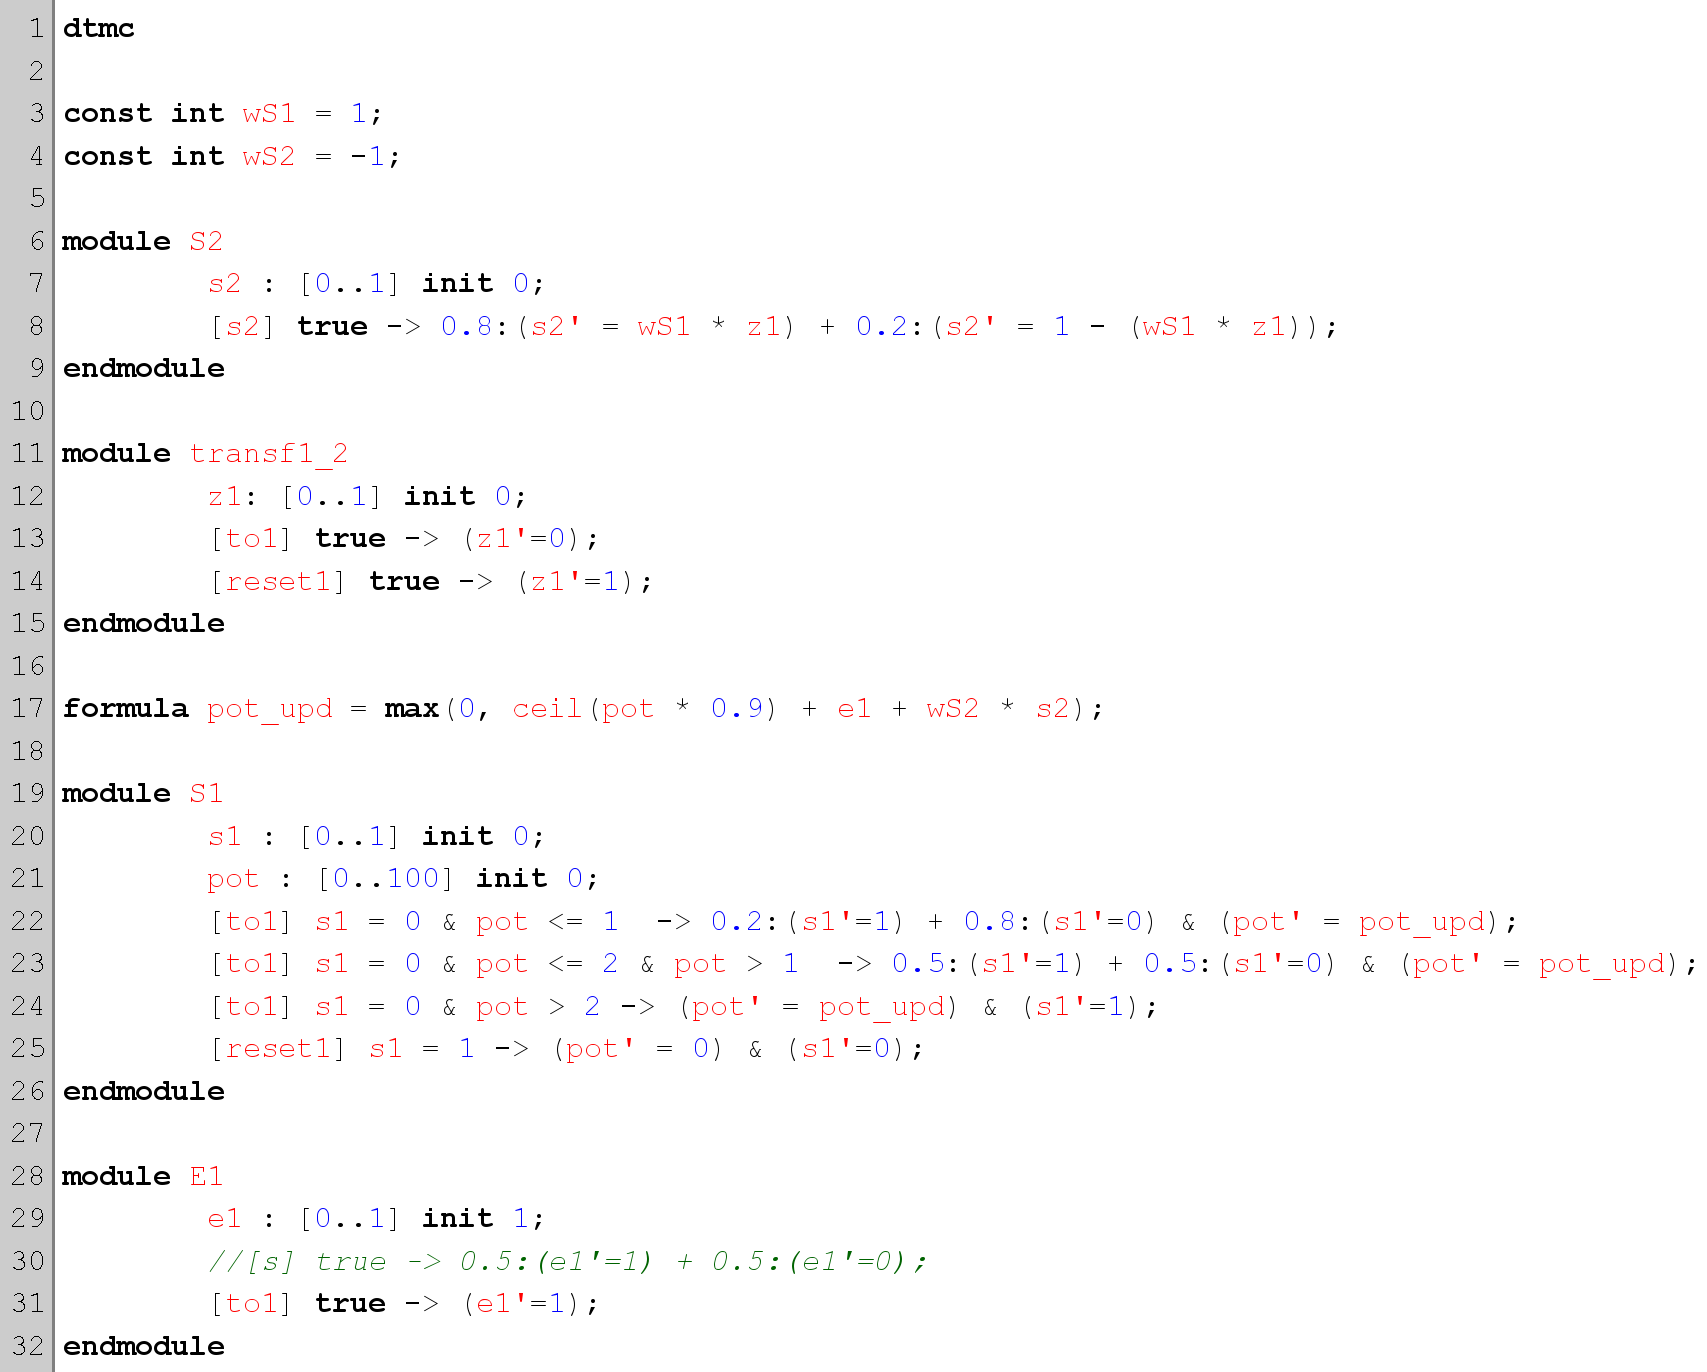
\includegraphics[width=0.75\textwidth]{pic/neg_loop_compl.png}
%   \end{figure}

% \end{frame}

